\section{X-Learning overview}
\label{sec:x_learning_overview}

X-Learning is a web platform for building e-learning systems. This platform build full-stack Javascript NodeJS API-centric HTML5 based Single Page Application with Web Components via Polymer Project. X-Learning is composed of guidelines, methodology and a library of elements. The document driven web development methodology and guidelines allow to build a very structured and usable Single Page Application. 
“Everything is an element, even a service” is the philosophy of the project. The joint use of Web Components and Strongloop Loopback framework following the document driven web development methodology allowed to create vertical widget that influence every level of the stack. With a descriptive implementation it is possible to give life to API, on the server side, and visual and functional widget on the client side. A Web Application is essentially built by composing elements together.

\begin{figure}[htb]
 \centering
 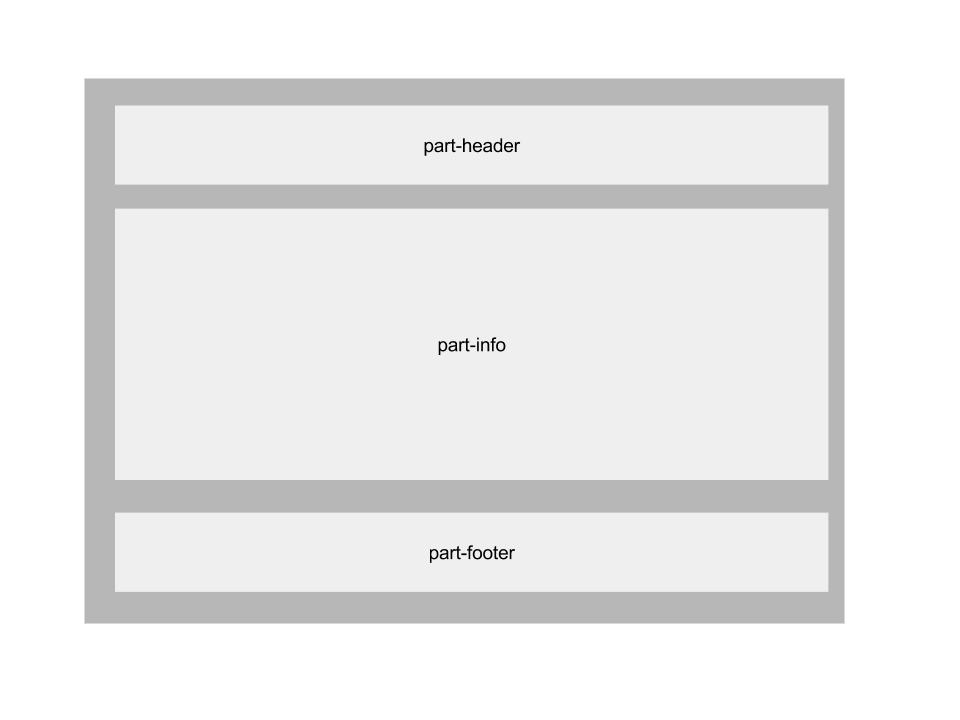
\includegraphics[width=1.0\linewidth]{images/chapter4/design-page.jpg}\hfill
 \caption[Design page]{Example of how the pages are designed}
 \label{fig:design_page}
\end{figure}

The Huge benefits coming from web components environment are reusability and access to reusable code.In X-Learning guidelines this pattern is applied to every kind of element.